\chapter{数据中心任务级传输优化模型}
\label{cha:mode-taskl}

\section{本章概述}
本章对数据中心任务传输模型进行介绍,首先,本章从数据中心非阻塞模型,以及传输任务等对数据中心任务级传输的模型进行介绍。
随后本章介绍数据中心任务调度问题的复杂度,最后,引入任务的离线调度算法,并证明离线调度算法的近似度。
\section{场景描述}
本章首先介绍数据中心网络的非阻塞结构的定义以及非阻塞结构的特性,
然后定义数据中心传输任务,以及介绍数据中心传输任务的特征。
\subsection{网络模型}
\begin{figure}[b]
\begin{center}
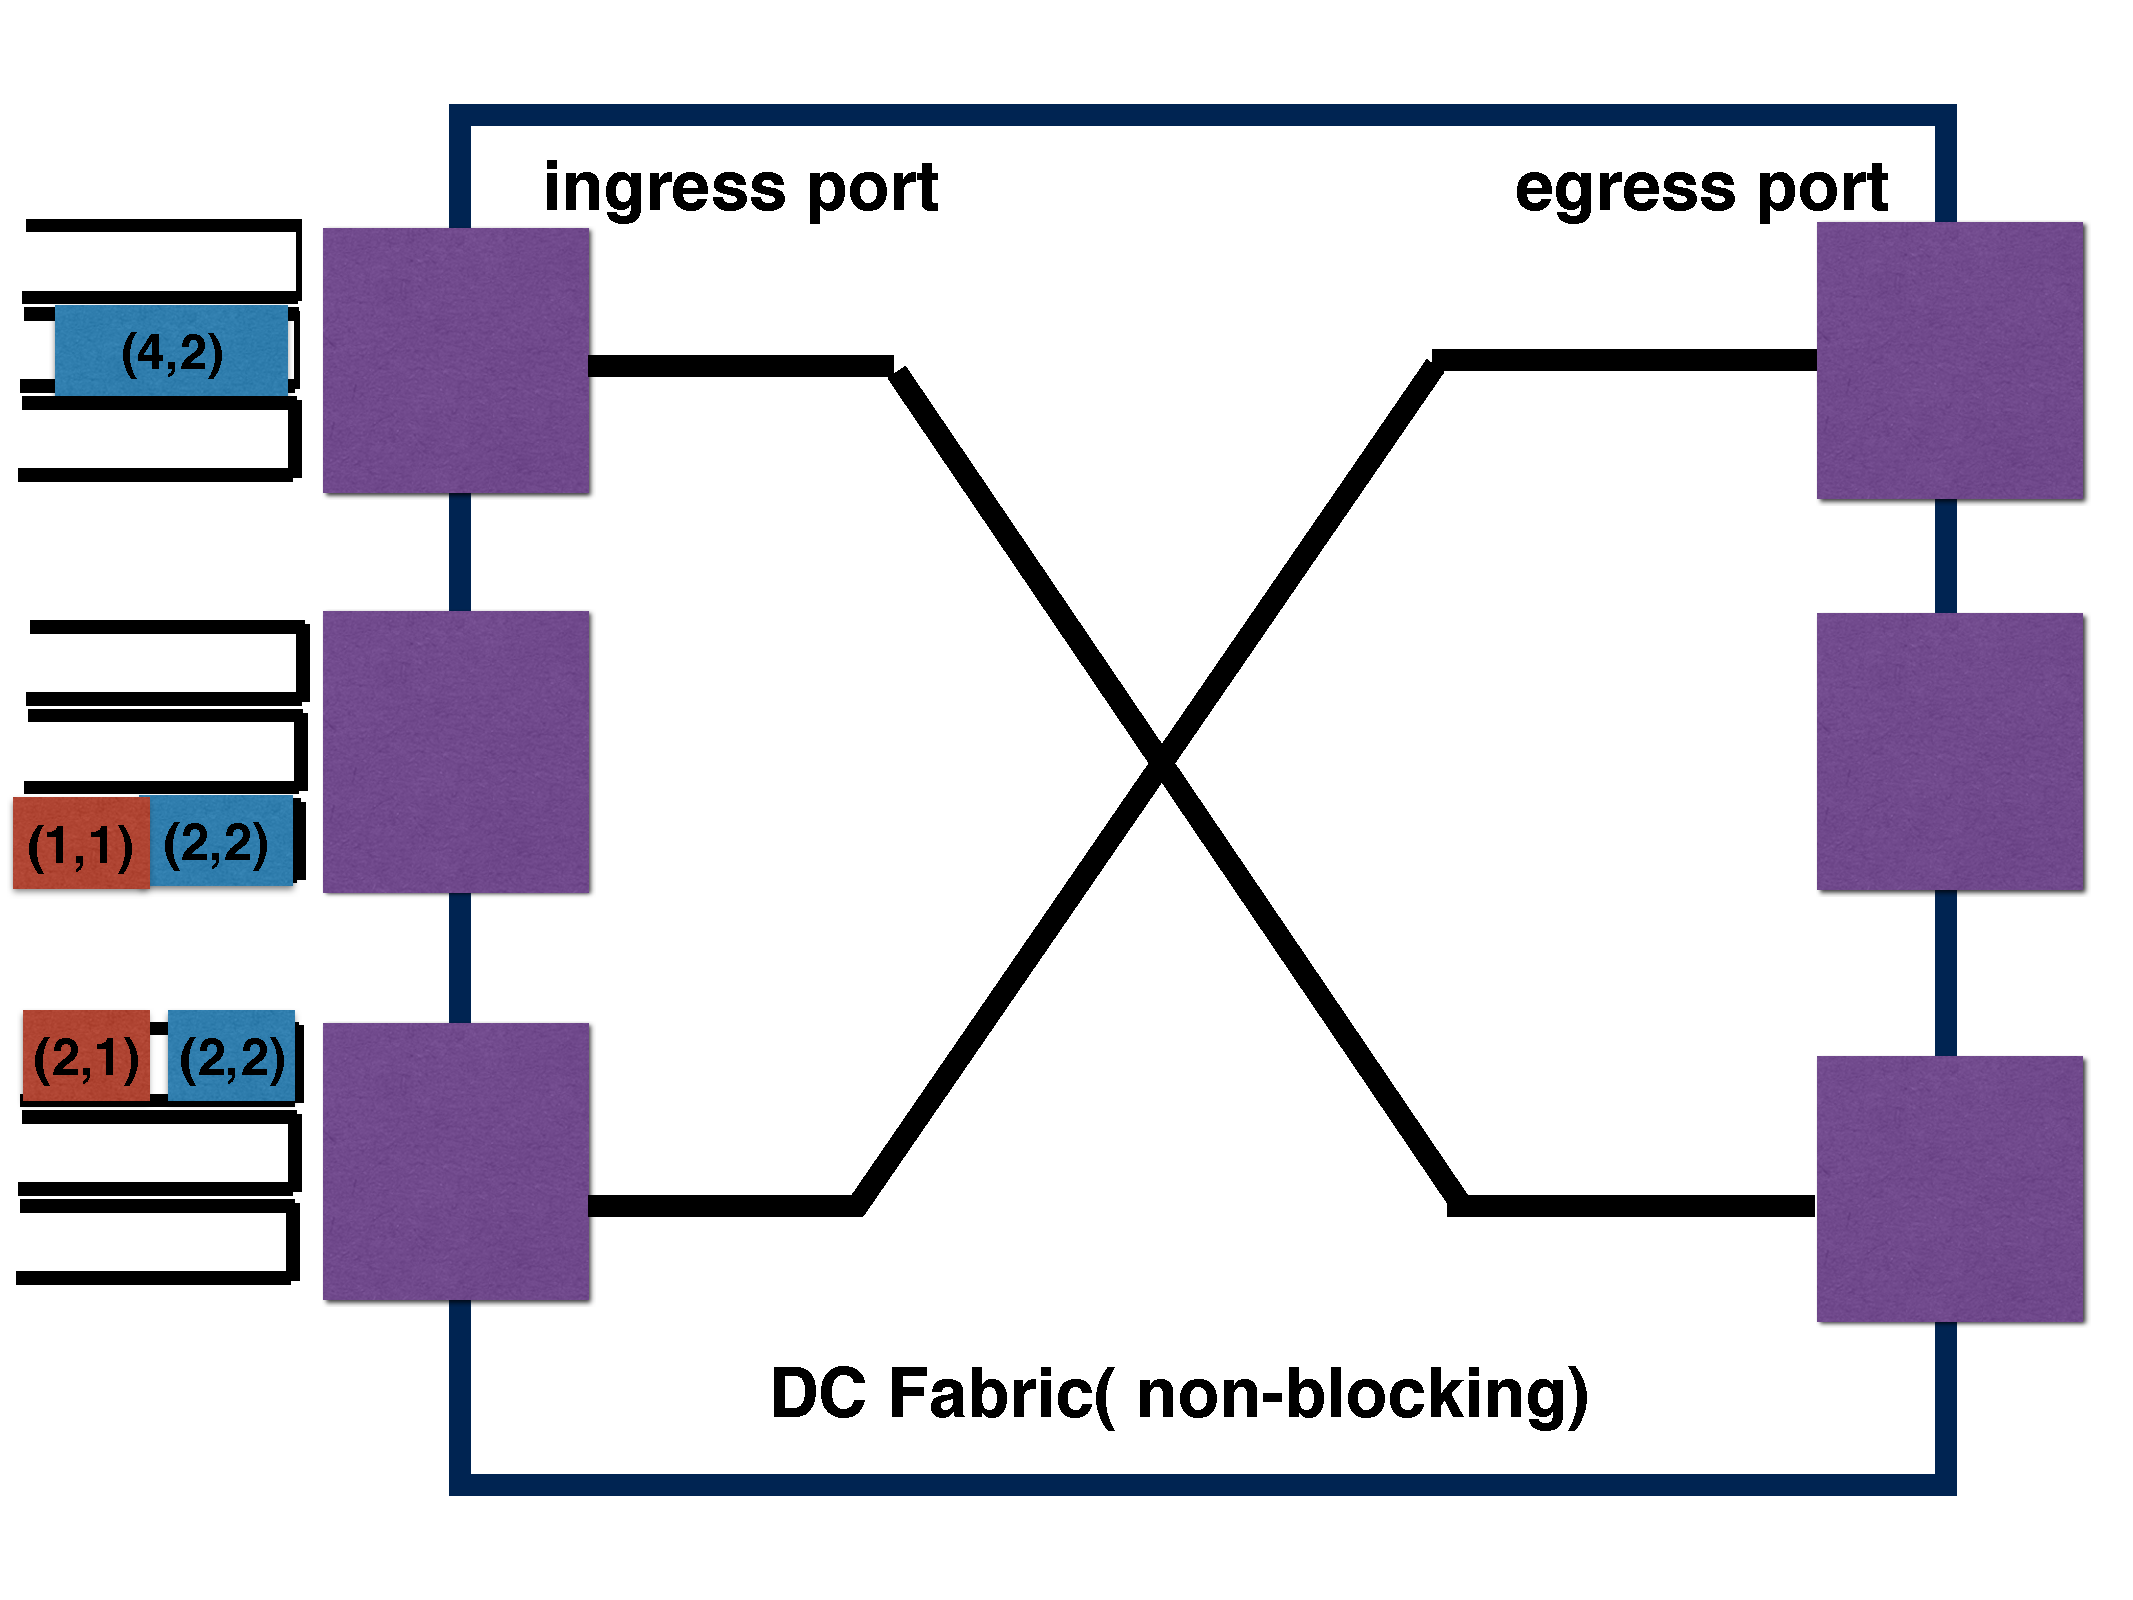
\includegraphics [width=0.9\columnwidth] {figures/DTARGET/picture/system/non-blocking.pdf}
\caption{非阻塞的数据中心体系结构}
\label{erasure-non-blocking-fig}
\end{center}
\end{figure}
最近的一些研究方法 \cite{pFabric,chowdhury2014efficient,huang2016sunflow,chowdhury2015efficient},
把数据中心当做一个大型交换机。
如图\ref{erasure-non-blocking-fig}所示,在非阻塞的网络模型中,所有的端口有统一的转发能力,
此外,在此网络模型中,所有的任务竞争交换机的入端口和出端口的带宽。
在本体系结构下,数据中心的内部没有任务的竞争,
只需要在入端口和出端口对任务进行优先级调度即可。
在后面的讨论中,为了简化问题,基于非阻塞体系结构讨论数据中心任务的调度。


\subsection{传输任务的定义}
在本部分,定义数据中心的传输任务,
数据中心的传输任务被定义为流组(coflow)\cite{chowdhury2014efficient},
流组是数据流的集合,这些流有共同的目标或者共同需要满足一定的期限等\cite{chowdhury2012coflow,chowdhury2014efficient}。
考虑在$t=0$时,数据中心同时开始传输 $n$条流组(coflow),
在非阻塞的网络体系结构下,假设数据中心有$m$台主机,
对应在非阻塞的网络体系结构下有$m$个入端口和$m$个出端口。

下面给出数据中心流组的定义:
 \begin{definition}\label{defination-coflow}
第k个流组(coflow)$F^{(k)}$,数学上定义为:$F^{(k)}=\{f^k_{i,j}|1 \leq i\leq m,1\leq j \leq m\}$,
$f^k_{i,j}$是每条流的长度(标准化后),机器$i$到机器 $j$。
其中$k$是coflow的序号。
\end{definition}


为了进一步简化问题,假设此“大型交换机”的入端口和出端口的带宽都是1(标准化后)。
所以,当只有这一条coflow进行传输时,传输时间是$f^k_{i,j}$ 。
在数据中心中,并不是每一条coflow都有$m\times m$条并行的数据流,
如果从机器$i$到$j$没有数据传输,那么$f^k_{i,j}=0$。
下面定义coflow的长度和宽度,

 \begin{definition}\label{defination-length}
coflow k的长度\textbf{length($F^{(k)}$)}=$\max \limits_{1 \leq i\leq m,1\leq j \leq m}\{ f^k_{i,j}\}$,即coflow中传输时间最长的数据流
\end{definition}



 \begin{definition}\label{defination-width}
定义$b^k_{i,j}$为第k条coflow的是否有从机器i到机器j数据传输的标记,
如果$f^k_{i,j}\ne 0$,那么$b^k_{i,j}=1$,否则$b^k_{i,j}=0$。
coflow的宽度为:\textbf{width($F^{(k)}$)}=$\sum_{i=1}^m\sum_{j=1}^mb^k_{i,j}$,
即coflow k,$F^{(k)}$的宽度为coflow中最大并行的流的数量。
\end{definition}


\section{传输任务的离线调度模型}
本部分中,首先讨论开放并行商店问题(concurrent open shop problem,简称COSP),
然后讨论数据中心的任务调度的问题复杂度,
最后,引入一个解决数据中心传输任务离线调度问题的调度算法,
并且讨论此算法的近似度。

\subsection{开放并行商店问题}\label{concurrent-open-shop}
开放并行商店模型的定义如下。
考虑一组机器M=\{1,2,...m\},每个机器可以处理一种类型的操作。
定义任务集合N=\{1,2,..n\},每个任务有m个子任务需要完成,
每个机器处理一个子任务。
机器之间相互独立。
当所有机器上的子任务完成时,此任务完成。
设$C_j$表示第j个任务的完成时间。
设置$w_j$为第j个任务的权重,
问题的优化目标为$\mathop {\min }\sum_{j=1}^n w_j\times C_j$

使用 $w_k$表示coflow的权重,权重在实际当中可以表示为coflow $F^{(k)}$的重要性,$C_k$为coflow k的完成时间,
定义如下的 理想化权重流组完成时间优化问题(Idealized Weighted Coflow Completion Time Minimization,简称IWCCTM) 问题:

\begin{eqnarray}
& {\rm minimize} & \sum_{k=1}^{n} w_{k} C_{k} \label{eq:WCCO-SC} \\
& {\rm s.t.} &\forall k,j:  \sum_{\forall l:C_l \leq C_k}\sum_{i=1}^{m}f_{i,j}^{(l)} \leq C_k  \label{eq:ingress_constraint}\\
&&\forall k,i: \sum_{\forall l:C_l \leq C_k}\sum_{j=1}^{m}f_{i,j}^{(l)} \leq C_k   \label{eq:egress_constraint}
\end{eqnarray}

IWCCTM目标是最小化权重流组完成时间之和,
其中(\ref{eq:ingress_constraint})和(\ref{eq:egress_constraint})是对入端口和出端口有带宽的限制。
对于一个coflow $F^{(k)}$,完成时间是$C_k$,考虑在$F^{(k)}$完成之前的流组(coflow)的集合:$F^{(l)}$:$C_l \le C_k$。
对于任意的入端口 $i$ (或者出端口$j$),在这个端口上的所有流的传输时间,
至少为:$\sum_{j=1}^{m}f_{i,j}$ (出端口 $j$上的为:$\sum_{i=1}^{m}f_{i,j}$),这个值应该小于$C_k$。
下面证明在只允许非抢先调度的情形下,任务的权重完成时间之和的问题是NP-hard的。

\subsection{NP-hard证明}
在本部分中,证明,在只允许非抢先调度的情形下,任务的权重完成时间之和的问题是NP-hard的。

 \begin{lemma}\label{IWCCTM-proof2}
 如果只允许非抢先调度,那么IWCCTM问题和开放商店中任务的权重完成时间之和的问题是等价的,问题的复杂度是NP-hard。
\end{lemma}

\begin{proof}
开放商店可以被描述为:有一系列的机器 $M = \{1,...,m\}$,
每台机器能执行一种类型的操作,
任务集合表示为$N = \{1,...,n\}$,每个任务需要特定的$m$类的操作。
每个任务 $j \in N$有一个权重$w_j \in R > 0$,并且任务$j$在机器$i$ 上的处理时间是$p_{ij} \in R\ge0$。
当一个任务在机器上的所有操作都完成了,才能认为这个任务完成。
特别的,一个任务的所有的操作能够并行的处理。

对于一个$m \times m$的数据中心,根据定义(\ref{defination-coflow})可以得到一条coflow $F^{(k)}$,
聚合每个端口发出的数据流,得到数据中心传输子任务的定义:

\begin{equation}
\label{coflow-subtask}
 L_l^{(k)}=\left\{
\begin{array}{rcl}
\sum_{i=1}^{m}f_{i,l}^{(k)}& {0      \le l   <m} \\
\sum_{j=1}^{m}f_{l-m,j}^{(k)} & {m      \le l   <2m} \\
\end{array} \right. 
\end{equation}

因为数据中心有$2m$个端口,因此每个流组有$2m$个传输子任务。
考虑开放商店中有$n$ 个任务和$2m$台转发能力相同的机器,每个任务有$2m$个子任务,每个子任务需要在一台机器上执行。
每个流组可以和每个任务对应,每台机器的子任务执行和每个传输子任务对应。
因为已经被证明,在开放商店中最小化任务权重完成时间是NP-hard\cite{mastrolilli2010minimizing}\cite{chen2000supply}\cite{roemer2006note}\cite{Qiu2016Experimental},
因此,在非阻塞网络中对流组的调度问题的复杂度也是NP-hard。
\end{proof}


\subsection{离线算法}
对于在开放商店中解决任务权重完成时间,
当前最优的解决方法是2-近似的贪心策略\cite{mastrolilli2010minimizing,kumar2011lp}。
因为IWCCTM问题和开放商店任务权重完成时间有很近的关系,
引入一个如算法\ref{IWCCM-offline}所示的离线非抢先调度算法。




\begin{algorithm}
\KwIn{Coflow 集合 $\mathcal{F}=\{F^{(k)}\}$,权重集合$\mathcal{W}=\{\overline{w_k}=w_k\}$, $1 \le k \le n$; } 
\KwOut{a permutation $\gamma$ of $\{1, \dots, n\}$;}
$\mathcal{P} \gets \{1, \dots, 2m\}$, $\mathcal{R} \gets \{1, \dots, n\}$\;
 $L_i^{(k)}= \sum_{j=1}^mf_{i,j}^{(k)}$  for $1 \le k \le n$ and $i \le m$\;
  $L_{j+m}^{(k)}= \sum_{i=1}^mf_{i,j}^{(k)}$ for $1 \le k \le n$ and $ j \le m$\;
 $L_p=\sum_{1 \le k \le n}L_p^{(k)}$ for each $p \in \mathcal{P}$\;
   \For{$i$ from $n$ to $1$ }{
   $p^*=\arg \max \limits_{p \in \mathcal{P}}L_p$\;
    $\gamma[i]=r^*=\arg\min \limits_{r \in \mathcal{R}} \overline{w_r}/L_{p^*}^{(r)}$\;
     $\theta=w_{r^*}/L_{p^*}^{(r^*)}$\;
     $\mathcal{R} = \mathcal{R} \setminus \{r^*\}$\;
    $\overline{w_r} = \overline{w_r}-\theta \times L_{p^*}^{(r)}$ for all $r \in \mathcal{R}$\;
    $L_p=L_p-L_p^{(r^*)}$ for all $p \in \mathcal{P}$\;
  }
  \textbf{return} $\gamma$;
  \caption{解决IWCCM的2近似算法}
  \label{IWCCM-offline}
 \end{algorithm}
 
 
 算法\ref{IWCCM-offline}首先构造了端口集合 $\mathcal{P}=\{1, \dots, 2m\}$,
 这个集合对应着非阻塞网络体系结构的“巨型交换机”的$m$个入端口和$m$个出端口,
 行1$\sim$4,计算了每个端口的负载。
 然后算法迭代的找出第i个循环下要调度的流组(coflow),循环是按照倒叙进行。
 在每轮迭代中,首先找出负载最重的端口$p^*$,然后找到这个端口上有最小的权重和负载比的流组(coflow),
 保存这个流组(coflow)的负载到$\gamma[i]$(行 6 $\sim$ 7),
 随后更新要调度的coflow的集合,以及要调度的coflow集合的权重,和端口的负载(行8 $\sim$ 11),
 随后,进行下一轮的迭代。
 
 可以很明显的看出,算法\ref{IWCCM-offline}产生序列$\gamma$ 的复杂度是$O(n(m+n))$,
 其中m是数据中心中端数量,n是任务的数量。
 
 \subsection{离线算法($2-\frac{2}{n+1}$)-近似证明}
 本部分,证明算法\ref{IWCCM-offline}的是2-近似,根据Chen\cite{chen2000supply},
 IWCCM中有如下限制:
 \begin{eqnarray}
  &\forall j \leq 2m, S \subset F: \sum_{k=1}^{|S|} L_{j}^{(k)} C_{k} \geq \frac{1}{2}\sum_{k=1}^{|S|} (L_{j}^{(k)})^2+ \frac{1}{2}(\sum_{k=1}^{|S|} L_{j}^{(k)})^2
\end{eqnarray}
其中F是要调度的coflow的集合,$L_{j}^{(k)}$是coflow k 在端口j的传输时间,
$|S|$是集合S的长度,因此,IWCCM可以表述为:
 \begin{eqnarray}
 & {\rm minimize} & \sum_{k=1}^{n} w_{k} C_{k} \label{eq:WCCO-SC2} \\
& {\rm s.t.} &\forall j \leq 2m, S \subset F: \sum_{k=1}^{|S|} L_{j}^{(k)} C_{k} \geq \frac{1}{2}\sum_{k=1}^{|S|} (L_{j}^{(k)})^2+ \frac{1}{2}(\sum_{k=1}^{|S|} L_{j}^{(k)})^2  \label{eq:IWCCM-SC3}
\end{eqnarray}

基于此,得到IWCCM的对偶函数为:
 \begin{eqnarray}\label{IWCCTM4}
 & {\rm maximize} & \sum_{j=1}^{2m}\sum_{S\subset F}\left [\frac{1}{2}\sum_{k=1}^{|S|} (L_{j}^{(k)})^2+ \frac{1}{2}(\sum_{k=1}^{|S|} L_{j}^{(k)})^2 \right ] y_j^S\label{eq:WCCO-SC4} \\
& {\rm s.t.} & \forall k\leq n:\sum_{j=1}^{2m} L_{j}^{(k)} \sum_{S\subset F:k=1}^{|S|} y_j^S=w_k  \label{eq:IWCCM-SC5}\\
& & \forall  y_j^S\geq 0  \label{eq:IWCCM-SC6}
\end{eqnarray}

为了证明算法\ref{IWCCM-offline}的是2-近似,引入以下引理:
 \begin{lemma}\label{IWCCTM-proof3}
 对任意的j$\leq $2m和S$\subset$F,有($\sum_{k=1}^{|S|}L_{j}^{(k)})^2\leq (2-\frac{2}{n+1})\left [ \frac{1}{2}\sum_{k=1}^{|S|} (L_{j}^{(k)})^2+ \frac{1}{2}(\sum_{k=1}^{|S|} L_{j}^{(k)})^2 \right ]$
\end{lemma}

基于此,有如下定理:

 \begin{theorem}\label{IWCCTM5}
 算法\ref{IWCCM-offline}的近似度是$(2-\frac{2}{n+1})$,其中n是并行的coflow的数目
 \end{theorem}

\begin{proof}
使用$p(i)$表示在第6行中第i个循环中中选出的端口,
使用$\theta(i)$表示在第8行中第i个循环计算的$\theta$值,
使用$\overline{w_r(i)}$表示第10行中第i个循环中调整的权重,
使用$\gamma(i)$表示第i循环起始时没有调度的coflow集合。
%%有$\gamma(i)=\{\bm{r^*(1)},\bm{r^*(2)}....\bm{r^*(i)}\}$,
有$\gamma(i)=\{r^*(1),r^*(2)...r^*(i)\}$,
其中$r^*(i)$表示coflow的id,
定义如下的对偶解,对于任意的j$\leq $2m和S$\subset$F

\begin{equation}
\label{duiou}
 y_j^S=\left\{
\begin{array}{rcl}
\theta(i) &\text{j=p(i),S=$\gamma(i)$,i=1,2,3...n}\\
0 &\text{其它情况}\\
\end{array} \right. 
\end{equation}
(\ref{duiou})是(\ref{IWCCTM4})的对偶解,是因为:
\begin{eqnarray}\label{proof_equal}
\sum_{j=1}^{2m} L_{j}^{r^*(i)} \sum_{S\subset F} y_j^S
&\overset{(a)}{=}&\sum_{l=i}^{n}  L_{p(l)}^{r^*(i)} y_{r^*(l)}^S\nonumber \\
&\overset{(b)}{=}&\sum_{l=i}^{n}  L_{p(l)}^{r^*(i)} \theta(l)\nonumber \\
&\overset{(c)}{=}& w_{r^*(i)}-\overline{w_{r^*(i)}}\nonumber \\
&\overset{(d)}{=}&w_{r^*(i)}
\end{eqnarray}
(a) 成立是因为算法1是从n到1开始循环的, 因此第i个循环的计算结果可以通过i+1个循环到n个循环推算得到。
(b) 成立是因为有解(\ref{duiou})成立,
(c)成立是因为在第i个循环,r$\in \gamma(i)$有 
\begin{equation}
w_r^{(i)}=w_r-\sum_{l=k}^{n}L_{p(l)}^r\theta(l)
\end{equation}
(d)成立是因为对于任意的k=1,2..n,有$\overline{w_{r^*(l)}}=0$。
通过(\ref{proof_equal}),可以得知,解(\ref{duiou})满足(\ref{eq:IWCCM-SC5})。
此外,从算法\ref{IWCCM-offline}输入得知,$\overline{w_{r^*(l)}}$初始化值为权重初始值,
算法\ref{IWCCM-offline}第7行和第10行知,每个循环选出最小的权重负载比,
因此,第10行中,$\theta \geq 0$,因此公式(\ref{eq:IWCCM-SC6})成立。
下面证明算法\ref{IWCCM-offline}的近似度是$(2-\frac{2}{n+1})$。
注意,算法\ref{IWCCM-offline}调度的coflow满足:
$C_{\gamma[1]} \leq C_{\gamma[2]} \leq... C_{\gamma[n]}$,
根据步骤6,7,对所有的i=1,2,..n,有$C_{\gamma[i]}=\sum_{j=1}^i L_{p^*(i)}^{r^*(j)}$。
令$(C_k^{CP})_{k \in \mathcal{F}}$是最优解,$(C_k^{*})_{k \in \mathcal{F}}$是最优解向量。
调度的最优化解为:


\begin{align}\label{proof_optimization}
&\sum_{k=1}^{n} w_{k} C_{k}\nonumber \\
=&\sum_{k=1}^{n} (\sum_{j=1}^{2m} L_{j}^{(k)} \sum_{S\subset F} y_j^S )C_{k}\nonumber \\
=&\sum_{j=1}^{2m} \sum_{S\subset F} y_j^S\sum_{k \in S}L_{j}^{(k)}C_k \nonumber \\
=&\sum_{l=1}^{n} y_{p^*(l)}^{\gamma(l)}\sum_{g=1}^{l} L_{p^*(l)}^{g}C_g\nonumber \\
=&\sum_{l=1}^{n} y_{p^*(l)}^{\gamma(l)}\sum_{h=1}^{l} L_{p^*(l)}^{r^*(h)}C_{r^*(h)}\nonumber \\
\overset{(e)}{\leq} &\sum_{l=1}^{n} y_{p^*(l)}^{\gamma(l)}C_{r^*(l)}\sum_{h=1}^{l} L_{p^*(l)}^{r^*(h)}\nonumber \\
\overset{(f)}{=} &\sum_{l=1}^{n} y_{p^*(l)}^{\gamma(l)}(\sum_{h=1}^{l} L_{p^*(l)}^{r^*(h)})^2\nonumber \\
\overset{(g)}{\leq}& (2-\frac{2}{n+1})\sum_{l=1}^{n}y_{p^*(l)}^{\gamma(l)}\{ \frac{1}{2}\sum_{h=1}^{l} \left[L_{p^*(l)}^{r^*(h)}\right]^2+ \frac{1}{2}\left[\sum_{h=1}^{l} L_{p^*(l)}^{r^*(h)}\right]^2 \}\nonumber \\
\overset{(h)}{\leq}& (2-\frac{2}{n+1}) \sum_{k=1}^{n} w_{k} C_{k}^{CP} \nonumber \\
\leq& (2-\frac{2}{n+1}) \sum_{k=1}^{n} w_{k} C_{k}^{*} 
\end{align}

(e)成立因为对于h=1,2,...l,有$C_{r^*(h)}\leq C_{r^*(l)} $,(f)成立,因为$C_{r^*(l)}=\sum_{h=1}^{l} L_{p^*(l)}^{r^*(h)}$,
(g)成立因为有引理\ref{IWCCTM-proof3}成立,(h)成立因为y是(\ref{IWCCTM4})$\sim$(\ref{eq:IWCCM-SC6})的解。
因此算法\ref{IWCCM-offline}的近似度是$(2-\frac{2}{n+1})$,其中n是并行的流组的数目
\end{proof}

\section{本章小结}
在本章中,介绍了数据中心任务级传输优化模型,
首先介绍了数据中心非阻塞模型,随后证明了数据中心流组(coflow)调度问题的复杂度,
最后提出了一个2-近似算法并证明算法的近似度。